\documentclass[conference]{IEEEtran}
\usepackage[T1]{fontenc}
\usepackage[utf8]{inputenc}
\usepackage{amsmath,amssymb,booktabs,graphicx,url}
\usepackage[hidelinks]{hyperref}
\hypersetup{pdftitle={Auditing Temporal Attention in Network Traffic Forecasting},pdfauthor={Anonymous Research Draft},pdfsubject={Reproducible recovered-data case study},pdfkeywords={network traffic forecasting, temporal attention, explainable AI}}
\graphicspath{{../figures/}}
\title{Auditing Temporal Attention in Network Traffic Forecasting:\\A Recovered-Data Case Study}
\author{\IEEEauthorblockN{Anonymous Research Draft}}
\begin{document}
\maketitle
\begin{abstract}
Temporal attention is frequently visualized as an explanation of a neural forecast, but predictive performance and input attribution are distinct properties. We reconstruct a network-traffic forecasting experiment from archived notebooks and a CESNET-derived aggregate containing 40,298 observations. Five timestamp discontinuities motivate a continuity-aware protocol that preserves observed targets and compares all models on 5,806 identical held-out origins. Persistence, seasonal naive and Ridge controls are evaluated alongside matched residual LSTMs with last-state, uniform, bounded-attention and learned-attention pooling, using three training seeds and 10- and 60-minute horizons. At 10 minutes, learned attention achieves mean MAE 10.34 GB, compared with 8.87 GB for Ridge and 10.35 GB for persistence. A separate audit compares attention rankings with Integrated Gradients, occlusion, recency and random rankings under two block replacements. For three replaced two-hour blocks, attention ranking produces a mean prediction change of 9.85 GB versus 7.82 GB for random ranking under the training-profile replacement. Integrated Gradients fails numerical completeness checks on some cases and is treated as provisional. The study provides a reproducible protocol and a bounded empirical account of attention behavior, rather than a new architecture, causal explanation or cross-network performance claim.
\end{abstract}
\begin{IEEEkeywords}
network traffic forecasting, explainable AI, temporal attention, Integrated Gradients, reproducibility
\end{IEEEkeywords}

\section{Introduction}
Forecasts of network demand can inform capacity planning and resource allocation. Statistical and recurrent approaches both remain relevant to this task, as surveyed by Oliveira Ferreira et al.~\cite{survey}. Model accuracy alone, however, does not establish whether a displayed explanation identifies the input history on which a forecast depends. This distinction matters when temporal attention is presented as an administrator-facing explanation.

This paper studies that distinction in a deliberately narrow setting: a single aggregate recovered from an unfinished traffic-forecasting project. Archived code already contained LSTM-attention experiments, but the original repository, upstream aggregation script and trained checkpoints were unavailable. Reusing the old metrics without reconstructing the evaluation protocol would obscure differences in target timestamps, preprocessing and model context. We therefore preserve the source artifacts, audit their data, and rebuild a controlled experiment.

Our questions are: (RQ1) does learned attention improve forecasting relative to simple controls and matched recurrent pooling alternatives? (RQ2) do its temporal rankings correspond to input-perturbation sensitivity, and are they stable across seeds and replacement choices? We contribute a documented recovery and continuity-aware evaluation, a matched pooling/context comparison, and a diagnostic explanation audit. We do not claim the first application of XAI to network forecasting: AICHRONOLENS already connects network forecasts with temporal explanations~\cite{aichronolens}. Nor do we infer human trust, operational benefit or causal importance from heatmaps.

\section{Related Work}
\subsection{Network Traffic Forecasting and Dataset Scope}
Network forecasting spans distinct targets, temporal scales and network granularities. Oliveira Ferreira et al.~\cite{survey} compare statistical and neural forecasting approaches, while Aouedi et al.~\cite{ntp_survey} organize deep-learning methods for network traffic prediction and discuss their practical challenges. These surveys support using explicit baselines and specifying the task before interpreting a model ranking. Lazaris and Prasanna~\cite{network_lstm} forecast fine-grained Tier-1 ISP traffic with LSTMs and group similar series to reduce the number of models. Their sub-minute setting differs from our 10-minute aggregate; their errors cannot be compared numerically with ours.

CESNET-TimeSeries24 provides long-duration IP-, subnet- and institution-level measurements~\cite{cesnet}. Koumar et al.~\cite{cesnet_comparison} subsequently compare deep forecasting models on this dataset, emphasizing accuracy and computational efficiency across granularities. Babai et al.~\cite{which_deep} evaluate a broader collection of network forecasting methods across four traffic datasets, multiple timescales and horizons; we consulted the November 2026 revision, which is a preprint. Such work makes our scope limitation concrete: this study evaluates one recovered aggregate whose institution membership is unknown, rather than reproducing a full CESNET benchmark or establishing cross-network superiority.

\subsection{Attention and Forecasting Architectures}
The LSTM~\cite{lstm} provides our recurrent backbone. Additive alignment in sequence modeling~\cite{bahdanau} is an architectural antecedent of the scorer we audit, rather than evidence that its weights necessarily explain a traffic forecast. DA-RNN~\cite{darnn} separates input-feature selection from temporal attention over encoder states. Temporal Fusion Transformers (TFT)~\cite{tft} combine recurrent processing, feature selection, gating and attention for multi-horizon forecasting. These richer architectures show why an outcome for our small univariate pooling model should not be generalized to every attention-based forecaster.

PatchTST~\cite{patchtst} uses temporal patches and channel independence for long-horizon forecasting, whereas Zeng et al.~\cite{linear} demonstrate the competitiveness of simple linear alternatives on long-horizon benchmarks. Together, these works motivate strong simple controls and broader architecture comparisons, without predicting the winner on our shorter horizons. The recovered PatchTST- and TFT-named notebooks are historical artifacts, not completed matched implementations of those published models; neither architecture is claimed as an evaluated comparator here.

\subsection{Explainability for Network Forecasting}
AIChronoLens connects explanations with temporal properties of mobile-network forecasting inputs~\cite{aichronolens}. Its journal extension~\cite{aichronolens_journal} also studies using explanatory information to diagnose and mitigate forecast errors. DeExp~\cite{deexp} examines influential base stations and model vulnerabilities under adversarial changes in spatiotemporal mobile forecasting. These are direct precedents for XAI in networking, beyond generic saliency work. Our experiment has neither spatial base-station structure nor an adversarial-attack protocol, so its two-hour replacements must not be presented as a reproduction of DeExp or as an operational vulnerability assessment.

\subsection{Faithfulness, Temporal Dependence and Numerical Reliability}
Attention's explanatory status remains a question of definition and evaluation. Jain and Wallace~\cite{attention_not} identify limitations of attention as attribution in NLP; Wiegreffe and Pinter~\cite{attention_notnot} motivate tests including uniform weights and seed variation. Bari\'c et al.~\cite{attention_benchmark} more directly benchmark attention-based interpretability in multivariate time-series forecasting using synthetic processes with known interactions, separating prediction accuracy from interpretability correctness. Their setting supports testing these properties independently; our real aggregate supplies no known ground-truth causal attribution.

Ismail et al.~\cite{ts_benchmark} benchmark saliency across time-series architectures and introduce temporal saliency rescaling to address conflated time and feature importance. Adebayo et al.~\cite{sanity} show why visually plausible saliency alone is insufficient and propose model/data randomization tests. Our seed, uniform-weight and perturbation diagnostics are not those randomization tests, and we do not claim to have run them. Yeh et al.~\cite{infidelity} distinguish fidelity and sensitivity through formal evaluation measures; our prediction-shift measure is a replacement-dependent sensitivity diagnostic, not their infidelity objective or a human-usability score.

Integrated Gradients (IG)~\cite{ig} supplies a full-model attribution comparator, but its mathematical properties do not eliminate numerical integration error. Dynamask~\cite{dynamask} and learned perturbations~\cite{learned_perturbations} treat temporal dependence as part of the explanation problem, reinforcing why constant masking is only a limited control. TIMING~\cite{timing} studies directional temporal contributions, evaluation cancellation and temporally aware IG paths. We do not implement those methods or assume that a different path would cure the integration failures observed here. Reporting those failures is part of the audit, rather than evidence that IG is generally invalid.

Table~\ref{tab:literature} positions the study against selected close precedents. Its contribution is a reproducible, narrowly scoped audit of forecasting and explanation claims on recovered evidence, not a new forecasting architecture or the first XAI treatment of network traffic.

\begin{table*}[t]
\caption{Selected literature and the boundary of the present experiment. These are methodological precedents, not models all evaluated in our benchmark.}
\label{tab:literature}\centering\footnotesize
\begin{tabular}{p{3.3cm}p{5.1cm}p{8.0cm}}\toprule
Study & Relevant focus & Distinction from this case study\\\midrule
Lazaris--Prasanna~\cite{network_lstm} & LSTM forecasting of fine-grained ISP traffic & Different sampling scale and series grouping; no transferred performance claim.\\
Koumar et al.; Babai et al.~\cite{cesnet_comparison,which_deep} & Network forecasting comparisons, granularity and efficiency & Broader benchmark scope; our single aggregate does not establish general model superiority.\\
AIChronoLens~\cite{aichronolens,aichronolens_journal} & Explanations tied to temporal network-forecast properties & Direct network-XAI precedent; our focus is matched pooling and diagnostic sensitivity.\\
DeExp~\cite{deexp} & Spatiotemporal influence and adversarial vulnerabilities & No spatial base-station or attack experiment is performed here.\\
DA-RNN; TFT~\cite{darnn,tft} & Feature selection and temporal attention architectures & Our univariate scorer is simpler; its result cannot characterize these architectures.\\
Bari\'c et al.~\cite{attention_benchmark} & Prediction versus attention-interpretability correctness & Synthetic interactions provide reference structure absent from our recovered aggregate.\\
Ismail et al.; Enguehard~\cite{ts_benchmark,learned_perturbations} & Temporal saliency and learned perturbations & Our fixed block replacements are diagnostics, not validated temporal generative perturbations.\\
TIMING~\cite{timing} & Temporal IG paths and directional evaluation & Not implemented; numerical IG nonconvergence remains explicitly unresolved here.\\\bottomrule
\end{tabular}
\end{table*}

\section{Recovered Data and Audit}
The source archive contains a research outline, eight notebooks and six CSVs. Four notebooks concern forecasting, three similarly named XAI notebooks concern Unicauca classification, and one notebook is empty. Classification outputs are excluded. Candidate Westermo, Tcpreplay and CTU CSVs contain whole-flow byte totals. Assigning those totals to a flow's start time would not reconstruct interval throughput, so these files do not enter the core experiment. A VPN-feature CSV is also excluded.

The actual experiment uses two recovered files: \texttt{global\_bytes\_10min.csv} supplies \texttt{n\_bytes}, and \texttt{times\_10\_minutes.csv} supplies timestamps. These tables join one-to-one by \texttt{id\_time}. Only historical aggregate byte volume is an input feature; no institution-specific series or recovered flow-classification features are used. The series contains 40,298 positive finite byte values from 9 October 2023 to 14 July 2024 UTC. We express volume as decimal GB per recovered interval. The aggregate's upstream construction is missing; consequently, it is described as a \emph{recovered CESNET-derived aggregate}, not as a verified network-wide sum. Artifact hashes and a recovery manifest accompany the implementation.

\begin{figure}[t]
\centering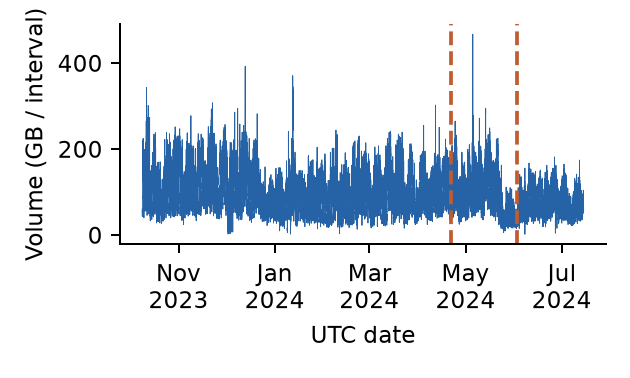
\includegraphics[width=\columnwidth]{series.png}
\caption{Recovered volume series. Dashed lines mark chronological split boundaries. Discontinuous windows are excluded, without fabricating observed targets.}
\label{fig:series}
\end{figure}

Five adjacent timestamp differences depart from 600 seconds: 4,200, 667, 956, 1,200 and 1,800 seconds. The records do not identify whether these arise from monitoring outages, clock behavior or another mechanism. We conservatively create a new contiguous segment at each departure. No interpolation, zero replacement, clipping or forward filling is applied. This differs from the archived Batch 4 notebook, whose resampling expanded the series to 40,308 bins and whose context-length runs evaluated different target sets. Archived metrics are retained as historical evidence only.

\section{Experimental Protocol}
\subsection{Targets and Temporal Splits}
Let $y_t$ denote observed interval volume and $o$ the index of the first unobserved interval. Inputs are $x_o=(y_{o-L},\ldots,y_{o-1})$; labels are $y_o$ and $y_{o+5}$. These represent the first and sixth future interval volumes, not a cumulative six-interval total. Forecasts are issued only after the final input interval is available.

The first $\lfloor0.70N\rfloor=28,208$ observations define training, the next $\lfloor0.15N\rfloor=6,044$ define validation, and the remainder define test. All labels for an origin must lie in its assigned split. Historical input may extend into the preceding split because it is available at forecast time. Mean and standard deviation are fit using training observations only.

Every comparator shares origins for which the interval from $o-1008$ through $o+5$ lies in one contiguous segment. The 1,008-step requirement makes the weekly seasonal control valid on identical timestamps. It is an eligibility rule, not the input length of every model. There are 24,402 training, 6,039 validation and 5,806 test origins. Test targets begin on 2 June and the final sixth-step target is on 13 July 2024 UTC; later gaps prevent another full weekly history. No model-specific target exclusions are allowed.

\subsection{Forecasting Models}
Persistence repeats $y_{o-1}$ at both horizons. Daily and weekly seasonal naive predictors use $y_{o+h-1-s}$ with $s\in\{144,1008\}$. Ridge regression takes 144 standardized lags and predicts both horizons directly. Its penalty is selected from $\{0.1,1,10,100\}$ by mean validation MSE; the selected value is 100.

Matched recurrent models use a single 32-unit LSTM~\cite{lstm}. Their pooling variants are the last hidden state, uniform mean pooling, learned additive attention and a recovered-style bounded scorer. For hidden states $h_t$, learned attention is
\begin{align}
 e_t&=v^\top\tanh(Wh_t+b), &
 \alpha_t&=\frac{\exp e_t}{\sum_j\exp e_j},\\
 c&=\sum_t\alpha_t h_t, &
 \hat{z}_{o,h}&=z_{o-1}+a_h^\top c+d_h.
\end{align}
The common persistence residual makes the architecture appropriate for short-term changes while exposing a distinct interpretation limit: attention weights describe the pooled hidden-state path, not the residual path. IG differentiates the complete model, including the residual.

The bounded scorer uses $e_t=\tanh(w^\top h_t+b)$, mirroring the scoring choice in the recovered notebook. Thus $e_t\in[-1,1]$ and $\alpha_i/\alpha_j\leq\exp(2)$. At $L=144$, the largest possible weight is at most $\exp(2)/(143+\exp(2))\approx0.049$. This is an architectural bound, not evidence that the observed weights reach it. The bounded model is a diagnostic reconstruction, not an exact TensorFlow reproduction. Learned attention is also trained at $L=288$ to test longer context on the same targets.

Each of five recurrent conditions uses seeds 42, 123 and 2026. All use Adam~\cite{adam} with learning rate 0.001, batch size 256, gradient-norm clipping at 1, a 40-epoch cap and patience six on mean standardized validation MSE, restoring the best checkpoint. No test-based configuration selection or retraining is performed. Computation uses four CPU threads on macOS arm64; exact library versions, training curves and checkpoints are included in the artifact.

\subsection{Metrics and Uncertainty}
We report MAE, RMSE and WAPE on the original GB scale, separately by horizon. Recurrent summaries use the mean and sample standard deviation over three seeds. Seed spread is not a confidence interval. For paired MAE contrasts, we average losses across seeds at each origin, then use 1,000 moving-block bootstrap replicates with a primary block length of 144 origins and sensitivity lengths 72 and 288. This is conditional uncertainty for the fitted models on one test period, not uncertainty across networks. First/middle/final thirds of the test period are also reported in the artifact.

\subsection{Explanation Audit}
We select 96 test origins evenly by order before inspecting errors. Horizon one is the planned explanation focus. Each 144-step history is grouped into 12 two-hour blocks. Rankings come from summed attention, summed absolute IG, single-block occlusion, recency and 20 random permutations. IG uses 32 trapezoidal integration intervals and a training-only local-time-of-day median profile; completeness residuals and a 64-interval check on 16 origins are recorded.

For the top $k\in\{1,3,6\}$ blocks, we replace inputs with the training time-of-day profile and measure absolute prediction change as well as change in absolute forecast error. A second replacement uses the constant training median while holding rankings fixed. Random effects are averaged over permutations before aggregation. Occlusion ranks are derived from the same perturbation family, so their strong deletion performance would not independently validate explanations. We also measure rank agreement, seed stability, normalized attention entropy and prediction change when learned weights are replaced with uniform weights while hidden states remain fixed.

All perturbations can be off-distribution. Large prediction change indicates sensitivity to a replacement, not causal importance; error can either increase or decrease. Attention weights cover hidden states that themselves mix earlier inputs. Accordingly, comparisons with raw-input attributions are diagnostics of interpretation claims, not tests of equality between mathematically identical quantities. Paired explanation-versus-random intervals resample UTC target days, with seed results averaged within the sampled groups.

\section{Results}
\begin{table*}[t]
\caption{Forecast errors in GB per interval on 5,806 common test origins. Recurrent values are mean $\pm$ sample standard deviation across three seeds. Deterministic baselines have one fit.}
\label{tab:forecast}\centering\small
\begin{tabular}{lrrrr}\toprule
 & \multicolumn{2}{c}{10 minutes} & \multicolumn{2}{c}{60 minutes}\\
Model & MAE & RMSE & MAE & RMSE\\\midrule
Persistence & 10.347 & 13.897 & 13.427 & 17.683 \\
Daily seasonal & 18.256 & 23.832 & 18.291 & 23.880 \\
Weekly seasonal & 21.778 & 28.245 & 21.783 & 28.248 \\
Ridge & 8.869 & 11.806 & 11.075 & 14.526 \\
LSTM last, 144 & 8.883 $\pm$ 0.046 & 11.802 $\pm$ 0.109 & 11.147 $\pm$ 0.186 & 14.681 $\pm$ 0.224 \\
Uniform, 144 & 10.354 $\pm$ 0.028 & 13.901 $\pm$ 0.026 & 13.282 $\pm$ 0.328 & 17.508 $\pm$ 0.350 \\
Bounded attn., 144 & 10.347 $\pm$ 0.013 & 13.893 $\pm$ 0.005 & 13.264 $\pm$ 0.160 & 17.422 $\pm$ 0.193 \\
Learned attn., 144 & 10.340 $\pm$ 0.004 & 13.893 $\pm$ 0.002 & 13.336 $\pm$ 0.040 & 17.567 $\pm$ 0.034 \\
Learned attn., 288 & 10.348 $\pm$ 0.002 & 13.900 $\pm$ 0.001 & 13.443 $\pm$ 0.009 & 17.689 $\pm$ 0.006 \\
\bottomrule\end{tabular}\end{table*}
\subsection{Predictive Performance}
Table~\ref{tab:forecast} reports every condition, including negative comparisons. At 10 minutes, learned attention has MAE 10.34 GB and RMSE 13.89 GB, versus 10.35 and 13.90 GB for persistence. Its MAE skill relative to persistence is 0.07\%. Ridge achieves MAE 8.87 GB and RMSE 11.81 GB. At 60 minutes, learned-attention MAE is 13.34 GB, persistence 13.43 GB and Ridge 11.07 GB. The lowest observed mean MAE among the evaluated conditions belongs to Ridge at 10 minutes and Ridge at 60 minutes; this is a descriptive ranking, not a test-selected retraining decision.

For learned attention minus Ridge at 10 minutes, the paired MAE difference is 1.47 GB, with primary moving-block interval [1.273, 1.673] GB. Against last-state pooling it is 1.46 GB [1.226, 1.689], against uniform pooling -0.01 GB [-0.024, -0.005], and against bounded attention -0.01 GB [-0.015, 0.002]. Negative differences favor learned attention. These contrasts average per-origin losses across seeds, not predictions from a seed ensemble.

\subsection{Context and Temporal Robustness}
Extending learned-attention context from 144 to 288 steps changes one-step MAE by 0.01 GB, with interval [0.003, 0.016] GB. Because both contexts share target timestamps, this comparison isolates context more cleanly than the archived runs, although optimization difficulty and model capacity remain possible mechanisms. Full 72/144/288-origin bootstrap sensitivity and test-period-third metrics are included in the artifact. The point estimates above are not substituted into the historical notebook result. Figures~\ref{fig:mae} and~\ref{fig:prediction} summarize errors and a fixed initial test episode.

\begin{figure*}[t]
\centering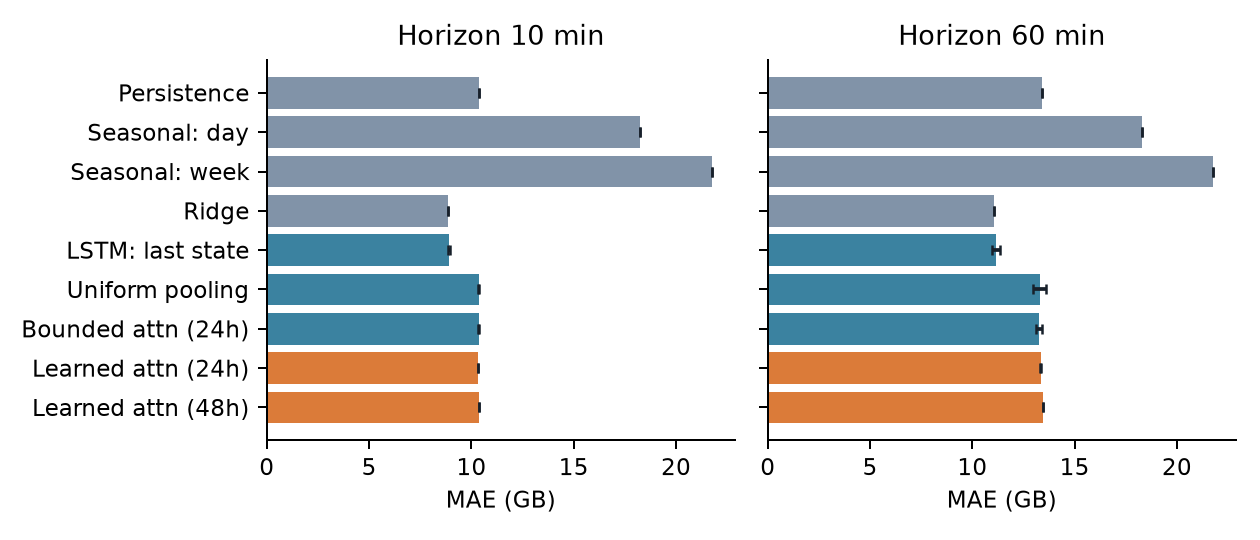
\includegraphics[width=\textwidth]{forecast_mae.png}
\caption{Forecast MAE on identical test origins. Recurrent error bars denote sample standard deviation over three seeds.}
\label{fig:mae}
\end{figure*}

\begin{figure}[t]
\centering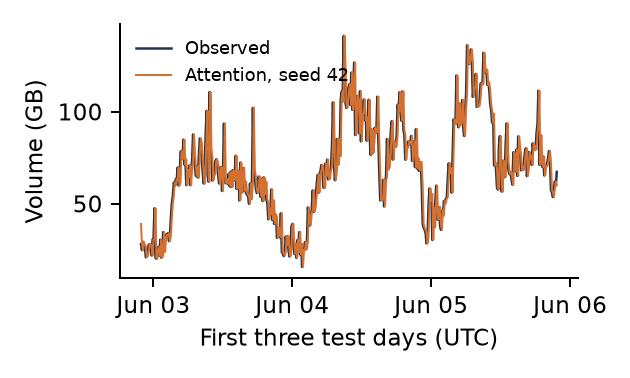
\includegraphics[width=\columnwidth]{forecast_example.png}
\caption{First three test days, shown without selecting a favorable error episode. One-step learned-attention predictions use seed 42.}
\label{fig:prediction}
\end{figure}

\begin{figure*}[t]
\centering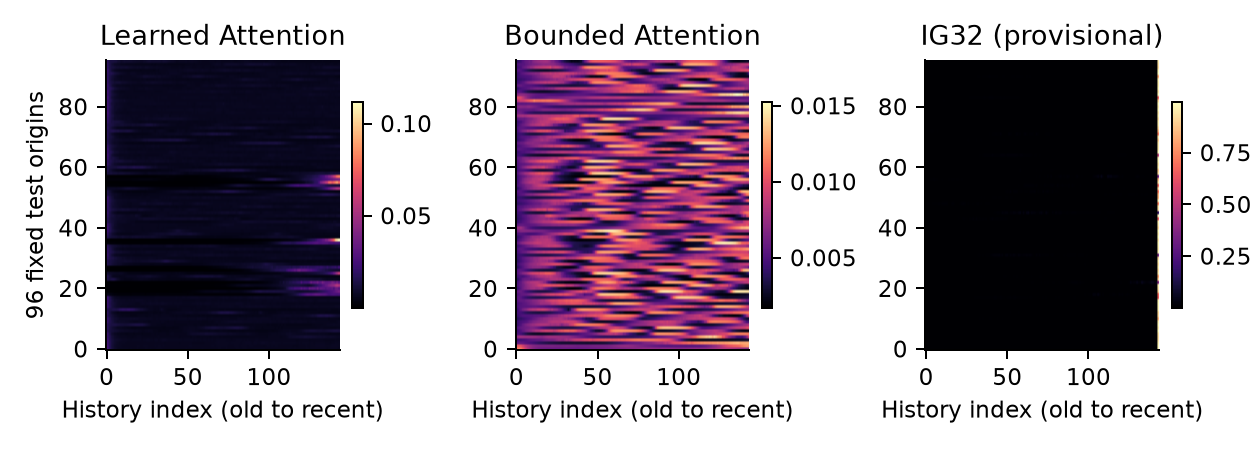
\includegraphics[width=\textwidth]{attribution_heatmaps.png}
\caption{Seed-42 temporal rankings at the 96 fixed origins. Each row is normalized for display; panels have separate color scales. IG includes the residual path and is provisional because numerical integration fails completeness checks in some cases.}
\label{fig:heatmaps}
\end{figure*}

\begin{figure*}[t]
\centering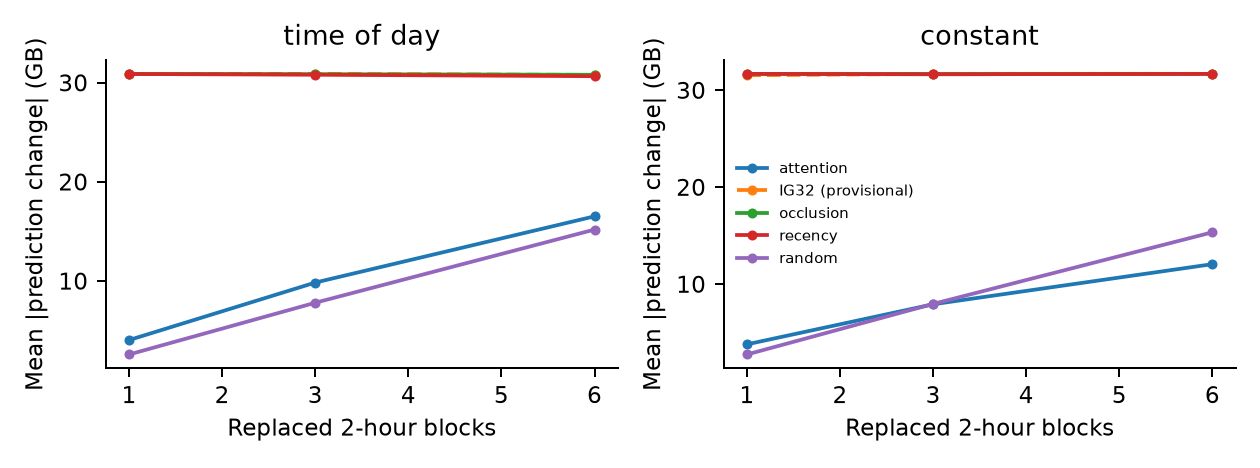
\includegraphics[width=\textwidth]{perturbation.png}
\caption{Learned-attention model: mean prediction shifts across the fixed origins and three seeds. Rankings are held fixed across replacements. The dashed IG32 comparator is provisional. Effects describe model sensitivity, not causal attribution.}
\label{fig:perturbation}
\end{figure*}

\section{Interpretability Analysis}
\subsection{Attention Concentration and Intervention}
Learned attention has mean normalized entropy 0.963, versus 0.986 for the bounded scorer (one indicates uniform weights). Mean maximum weight is 0.0226 for learned attention and 0.0119 for bounded attention. Replacing learned weights with uniform weights while holding hidden states fixed changes the one-step output by 0.19 GB on average. This measures sensitivity of the pooling path; it does not remove the residual contribution.

\subsection{Input Attribution and Perturbation}
IG32-based comparisons below are provisional because numerical completeness fails in some cases, as detailed in the numerical-reliability diagnostic. Across fixed origins and seeds, mean block-rank Spearman correlation is 0.469 for attention versus absolute IG and 0.421 for attention versus occlusion. Mean cross-seed attention-rank correlation is 0.710. The 32-interval IG mean absolute completeness residual is 0.4650 GB, with maximum 19.5263 GB. On the 16-origin numerical check, the 64-interval mean residual is 0.3065 GB. These numerical diagnostics are reported rather than assuming exact integration.

Replacing the top three two-hour blocks with the training time-of-day profile yields mean prediction shifts of 9.85 GB for attention ranking, 30.91 GB for IG, 30.87 GB for occlusion, 30.82 GB for recency and 7.82 GB for random ranking. Attention minus random has mean difference 2.04 GB and paired day-bootstrap interval [-0.091, 4.002] GB. The corresponding change in absolute forecast error is 5.98 GB for attention and 18.68 GB for IG; an error reduction after perturbation is possible and is not censored.

Under constant-median replacement with the same rankings, mean shifts are 7.93 GB for attention, 31.70 GB for IG and 7.97 GB for random order. Figure~\ref{fig:perturbation} shows the full 1/3/6-block curves. Sensitivity to replacement choice and the distinction between hidden-state weights and full-model input attribution limit a literal interpretation of the heatmaps in Fig.~\ref{fig:heatmaps}.

\subsection{Numerical Reliability of IG}
The planned IG checks reveal substantial numerical nonconvergence on some model/origin combinations. A secondary follow-up repeats integration at 128, 512 and 2,048 intervals on the same first 16 fixed origins for every model/seed. At 2,048 intervals, the largest absolute completeness residual is still 2.70 GB, and 3 of the six model/seed combinations contain at least one residual above 0.1 GB. Accordingly, IG32 rankings and all comparisons involving them are provisional, including correction-only IG correlations. We do not infer that attention is inferior to a numerically validated IG explanation. Occlusion, recency, random interventions and exact Ridge decomposition use direct model evaluations and do not depend on IG quadrature. The artifact retains the original IG outputs and all convergence diagnostics rather than silently replacing the planned method.

\subsection{Secondary Residual-Path Diagnostic}
As a secondary diagnostic added while primary training was in progress, after initial baseline outputs were available, we separate the pooled correction from the persistence path. Subtracting the exact linear residual attribution from full-model IG gives correction-only IG. Its mean block-rank correlation with attention is 0.539. Under three-block training-profile replacement, correction-only mean shifts are 0.20 GB for attention ranking, 0.23 GB for the original full-model IG ranking and 0.13 GB for random ranking. These retain the original rankings; the IG deletion comparator is not re-ranked using correction-only attribution. This path-aware diagnostic avoids interpreting a mismatch in computational scope as proof that attention fails to describe its own branch. It introduces no refitting and does not replace the planned full-model audit.

\subsection{Exploratory Linear Decomposition}
After inspecting baseline results, we added a post-hoc Ridge decomposition without refitting or changing the primary protocol. Relative to the training-mean reference, its prediction equals a constant plus the sum of lag-wise fitted contributions. The most recent lag has coefficient 0.413 at 10 minutes and 0.354 at 60 minutes. Reconstructed predictions agree with saved forecasts to within 0.00002 GB. Coefficients and all per-origin contributions are included in the artifact. Exact reconstruction explains the fitted linear computation; correlated lag coefficients are not causal effects.

\section{Discussion and Limitations}
The controlled experiment separates two decisions that are often conflated: whether an attention-based architecture predicts well, and whether the weights provide a reliable account of input influence. A model can be useful while a literal reading of its heatmap is misleading. Conversely, an explanation method can induce a large perturbation response without improving the unmodified forecast. These distinctions are particularly visible when a persistence residual supplies predictive information outside the displayed attention path.

The evaluation has material limits. First, upstream aggregate construction and institution membership are unavailable, so the source is CESNET-derived rather than independently verified as a specific public benchmark subset. Second, the study has one aggregate and one chronological holdout; seed repetitions do not create independent networks. Third, preserving observations and excluding discontinuities sacrifices coverage, including the end of the recording, in exchange for an explicit continuity assumption. Fourth, the shared weekly-history eligibility rule narrows the target population even for short-context models. Fifth, this finite model set does not establish state-of-the-art performance; published alternatives such as PatchTST, TFT or DA-RNN~\cite{patchtst,tft,darnn}, or a larger tuning study, could change predictive rankings.

The explanatory tests are likewise conditional on their baseline, grouping and horizon. A two-hour block hides finer distinctions, median replacement can yield unrealistic transitions, and IG depends on its reference path. Bootstrap intervals reflect finite observed days, not arbitrary deployment regimes; trends and nonstationarity can undermine their nominal coverage. Uniform-weight intervention is a model-internal sensitivity test. Attention conditioning, initialization and optimizer settings were not exhaustively tuned, so an unfavorable result under this fixed budget is not a universal failure of attention. None of these quantities measures administrator trust, explanation usability or causal mechanisms in the network. We therefore report agreement and disagreement without labeling an attribution method ground truth.

\section{Conclusion}
On identical held-out targets, learned attention obtains MAE 10.34 GB at 10 minutes and 13.34 GB at 60 minutes, compared with Ridge MAEs of 8.87 and 11.07 GB. The matched controls and direct perturbation diagnostics support assessing forecasting accuracy separately from the interpretation of attention weights. Numerical IG nonconvergence prevents treating its rankings as a validated reference here. The recovered-data artifact makes preprocessing, target eligibility and model comparisons inspectable, while preserving negative results and provenance limits. Future work should restore or independently regenerate aggregation provenance, evaluate multiple institutional series and chronological folds, and test richer temporal replacements~\cite{learned_perturbations,timing} and additional forecasting architectures. These extensions are necessary before broad operational or cross-network claims.

\section*{Reproducibility and Draft Status}
The accompanying artifact contains unmodified recovered sources, hashes, a pre-training protocol, executable experiment and analysis scripts, locked dependencies, all checkpoints, per-origin forecasts, diagnostic arrays and generated figures. Archived notebook outputs are explicitly separated from newly executed results. This anonymous manuscript is a research draft for review; author identities, data-release permissions and a target venue must be confirmed before submission.

\begin{thebibliography}{99}
\bibitem{survey} G. Oliveira Ferreira, C. Ravazzi, F. Dabbene, G. C. Calafiore, and M. Fiore, ``Forecasting Network Traffic: A Survey and Tutorial with Open-Source Comparative Evaluation,'' \emph{IEEE Access}, vol. 11, pp. 6018--6044, 2023, doi: 10.1109/ACCESS.2023.3236261.
\bibitem{aichronolens} C. Fiandrino, E. P\'erez G\'omez, P. Fern\'andez P\'erez, H. Mohammadalizadeh, M. Fiore, and J. Widmer, ``AIChronoLens: Advancing Explainability for Time Series AI Forecasting in Mobile Networks,'' in \emph{Proc. IEEE INFOCOM}, 2024, pp. 1521--1530, doi: 10.1109/INFOCOM52122.2024.10621134.
\bibitem{ntp_survey} O. Aouedi, V. A. Le, K. Piamrat, and Y. Ji, ``Deep Learning on Network Traffic Prediction: Recent Advances, Analysis, and Future Directions,'' \emph{ACM Computing Surveys}, vol. 57, no. 6, art. 151, 2025, doi: 10.1145/3703447.
\bibitem{network_lstm} A. Lazaris and V. K. Prasanna, ``An LSTM Framework for Modeling Network Traffic,'' in \emph{Proc. IFIP/IEEE IM Workshops (AnNet)}, 2019, pp. 848--853. \url{https://alazaris.github.io/assets/annet_2019.pdf}.
\bibitem{cesnet} J. Koumar, K. Hynek, T. \v{C}ejka, and P. \v{S}i\v{s}ka, ``CESNET-TimeSeries24: Time Series Dataset for Network Traffic Anomaly Detection and Forecasting,'' \emph{Scientific Data}, vol. 12, art. 338, 2025, doi: 10.1038/s41597-025-04603-x.
\bibitem{cesnet_comparison} J. Koumar, T. Smole\v{n}, K. Je\v{r}\'abek, and T. \v{C}ejka, ``Comparative Analysis of Deep Learning Models for Real-World ISP Network Traffic Forecasting,'' arXiv:2503.17410, 2025. \url{https://arxiv.org/abs/2503.17410}.
\bibitem{which_deep} E. M. A. Babai, A. M. A. Babai, and K. Okamura, ``Which Deep Learner? A Systematic Evaluation of Advanced Deep Forecasting Models Accuracy and Efficiency for Network Traffic Prediction,'' arXiv:2601.02694v2, 2026. \url{https://arxiv.org/abs/2601.02694v2}.
\bibitem{lstm} S. Hochreiter and J. Schmidhuber, ``Long Short-Term Memory,'' \emph{Neural Computation}, vol. 9, no. 8, pp. 1735--1780, 1997, doi: 10.1162/neco.1997.9.8.1735.
\bibitem{bahdanau} D. Bahdanau, K. Cho, and Y. Bengio, ``Neural Machine Translation by Jointly Learning to Align and Translate,'' in \emph{Proc. ICLR}, 2015. \url{https://arxiv.org/abs/1409.0473}.
\bibitem{darnn} Y. Qin, D. Song, H. Chen, W. Cheng, G. Jiang, and G. Cottrell, ``A Dual-Stage Attention-Based Recurrent Neural Network for Time Series Prediction,'' in \emph{Proc. IJCAI}, 2017. \url{https://arxiv.org/abs/1704.02971}.
\bibitem{tft} B. Lim, S. \"O. Ar\i k, N. Loeff, and T. Pfister, ``Temporal Fusion Transformers for Interpretable Multi-horizon Time Series Forecasting,'' \emph{International Journal of Forecasting}, vol. 37, no. 4, pp. 1748--1764, 2021, doi: 10.1016/j.ijforecast.2021.03.012.
\bibitem{patchtst} Y. Nie, N. H. Nguyen, P. Sinthong, and J. Kalagnanam, ``A Time Series Is Worth 64 Words: Long-term Forecasting with Transformers,'' in \emph{Proc. ICLR}, 2023. \url{https://arxiv.org/abs/2211.14730}.
\bibitem{linear} A. Zeng, M. Chen, L. Zhang, and Q. Xu, ``Are Transformers Effective for Time Series Forecasting?,'' in \emph{Proc. AAAI}, vol. 37, no. 9, 2023, pp. 11121--11128, doi: 10.1609/aaai.v37i9.26317.
\bibitem{aichronolens_journal} P. Fern\'andez P\'erez, C. Fiandrino, E. P\'erez G\'omez, H. Mohammadalizadeh, M. Fiore, and J. Widmer, ``AIChronoLens: AI/ML Explainability for Time Series Forecasting in Mobile Networks,'' \emph{IEEE Transactions on Mobile Computing}, vol. 24, no. 8, pp. 7757--7772, 2025, doi: 10.1109/TMC.2025.3554035.
\bibitem{deexp} S. Moghadas Gholian, C. Fiandrino, N. Vallina-Rodr\'iguez, M. Fiore, and J. Widmer, ``DeExp: Revealing Model Vulnerabilities for Spatio-Temporal Mobile Traffic Forecasting With Explainable AI,'' \emph{IEEE Transactions on Mobile Computing}, vol. 24, no. 6, pp. 5245--5263, 2025, doi: 10.1109/TMC.2025.3531544.
\bibitem{attention_not} S. Jain and B. C. Wallace, ``Attention is not Explanation,'' in \emph{Proc. NAACL-HLT}, 2019, pp. 3543--3556, doi: 10.18653/v1/N19-1357.
\bibitem{attention_notnot} S. Wiegreffe and Y. Pinter, ``Attention is not not Explanation,'' in \emph{Proc. EMNLP-IJCNLP}, 2019, pp. 11--20, doi: 10.18653/v1/D19-1002.
\bibitem{attention_benchmark} D. Bari\'c, P. Fumi\'c, D. Horvati\'c, and T. Lipic, ``Benchmarking Attention-Based Interpretability of Deep Learning in Multivariate Time Series Predictions,'' \emph{Entropy}, vol. 23, no. 2, art. 143, 2021, doi: 10.3390/e23020143.
\bibitem{ts_benchmark} A. A. Ismail, M. Gunady, H. Corrada Bravo, and S. Feizi, ``Benchmarking Deep Learning Interpretability in Time Series Predictions,'' in \emph{Advances in Neural Information Processing Systems}, vol. 33, 2020. \url{https://proceedings.neurips.cc/paper/2020/hash/47a3893cc405396a5c30d91320572d6d-Abstract.html}.
\bibitem{sanity} J. Adebayo, J. Gilmer, M. Muelly, I. Goodfellow, M. Hardt, and B. Kim, ``Sanity Checks for Saliency Maps,'' in \emph{Advances in Neural Information Processing Systems}, vol. 31, 2018. \url{https://arxiv.org/abs/1810.03292}.
\bibitem{infidelity} C.-K. Yeh, C.-Y. Hsieh, A. S. Suggala, D. I. Inouye, and P. Ravikumar, ``On the (In)fidelity and Sensitivity of Explanations,'' in \emph{Advances in Neural Information Processing Systems}, vol. 32, 2019. \url{https://arxiv.org/abs/1901.09392}.
\bibitem{ig} M. Sundararajan, A. Taly, and Q. Yan, ``Axiomatic Attribution for Deep Networks,'' in \emph{Proc. ICML}, PMLR 70, 2017, pp. 3319--3328.
\bibitem{dynamask} J. Crabb\'e and M. Van Der Schaar, ``Explaining Time Series Predictions with Dynamic Masks,'' in \emph{Proc. ICML}, PMLR 139, 2021, pp. 2166--2177.
\bibitem{learned_perturbations} J. Enguehard, ``Learning Perturbations to Explain Time Series Predictions,'' in \emph{Proc. ICML}, PMLR 202, 2023, pp. 9329--9342. \url{https://proceedings.mlr.press/v202/enguehard23a.html}.
\bibitem{timing} H. Jang, C. Kim, and E. Yang, ``TIMING: Temporality-Aware Integrated Gradients for Time Series Explanation,'' in \emph{Proc. ICML}, PMLR 267, 2025, pp. 26877--26895. \url{https://proceedings.mlr.press/v267/jang25a.html}.
\bibitem{adam} D. P. Kingma and J. Ba, ``Adam: A Method for Stochastic Optimization,'' in \emph{Proc. ICLR}, 2015. \url{https://arxiv.org/abs/1412.6980}.
\end{thebibliography}
\end{document}
